%
% radon.tex -- Radon transform
%
% (c) 2021 Prof Dr Andreas Müller, OST Ostschweizer Fachhochschule
%
\documentclass[tikz]{standalone}
\usepackage{amsmath}
\usepackage{times}
\usepackage{txfonts}
\usepackage{pgfplots}
\usepackage{csvsimple}
\usepackage{mathrsfs}
%\definecolor{polarcolor}{rgb}{1,0,0}
\definecolor{polarcolor}{rgb}{0,0,0}
\definecolor{pointcolor}{rgb}{0,1,1}
%\definecolor{dircolor}{rgb}{0,0.6,0}
\definecolor{dircolor}{rgb}{0.8,0,0}
\def\w{65}
\def\r{2.2}
\pgfmathparse{6.4*\w/180-3.2}
\xdef\wh{\pgfmathresult}
\usetikzlibrary{arrows,intersections,math}
\begin{document}
\def\skala{1}
\begin{tikzpicture}[>=latex,thick,scale=\skala]
\clip (-6.85,-3.3) rectangle (7.15,3.7);

\begin{scope}[xshift=-3.65cm]
	\node at (0,0) {
\includegraphics[width=6.4cm]{mathman.jpg}};
	\begin{scope}
		\clip (-3.2,-3.2) rectangle (3.2,3.2);
		\fill[color=dircolor!10!white,opacity=0.7]
			(0,0) -- (1.5,0) arc (0:\w:1.5) -- cycle;
		\draw[color=dircolor] (0,0) -- (1.5,0) arc (0:\w:1.5);
		\node[color=dircolor] at ({\w/2}:1) {$\varphi$};
		\draw[color=dircolor] ({\w+180}:5) -- ({\w}:5);
		\begin{scope}[rotate=\w]
		\foreach \d in {-5,-4.5,...,5}{
			\draw[line width=0.1pt,color=pointcolor] (\d,-5) -- (\d,5);
			\fill[color=pointcolor] (\d,0) circle[radius=0.03];
		}
		\end{scope}
	\end{scope}
\end{scope}

\begin{scope}[xshift=3.65cm]
\node at (0,0) {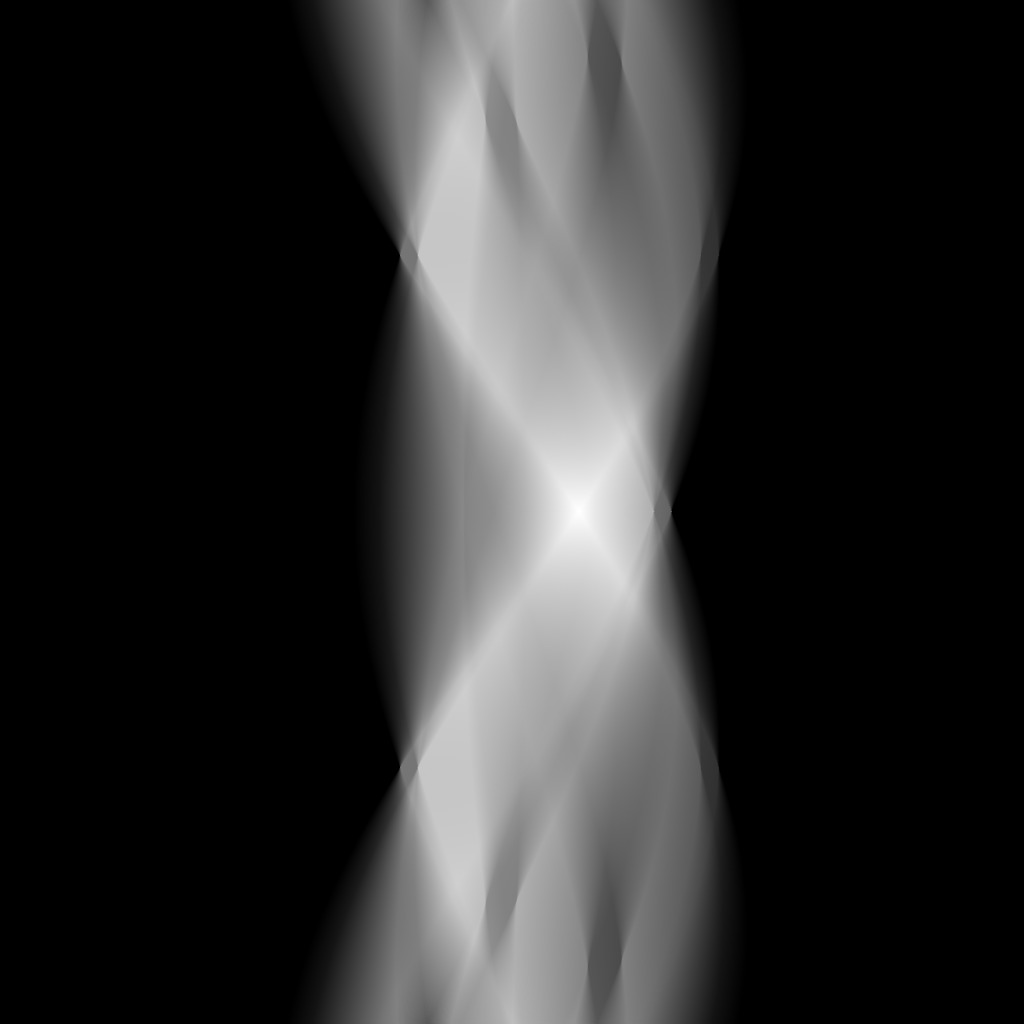
\includegraphics[width=6.4cm]{mathman-radon.jpg}};
	\draw[color=pointcolor] (-3.2,\wh) -- (3.2,\wh);
	\draw[->,color=polarcolor] (0,-3.2) -- (0,3.5)
		coordinate[label={right:$\varphi$}];
	\draw[->,color=polarcolor]
		(-3.2,-3.2) -- (3.4,-3.2) coordinate[label={$r$}];
	\fill[color=polarcolor] (0,-3.2) circle[radius=0.05];
	\foreach \y in {0,3.2}{
		\draw[color=polarcolor] (-0.05,\y) -- (0.05,\y);
	}
	\node[color=polarcolor] at (0,3.2)
		[below left] {$\scriptstyle \pi\mathstrut$};
	\node[color=polarcolor] at (0,0) [left] {$\frac{\pi}{2}\mathstrut$};
	\node[color=polarcolor] at (0,-3.2)
		[above left] {$\scriptstyle 0\mathstrut$};
	\node[color=dircolor] at (-3.2,\wh) [above right] {$\varphi$};
\end{scope}

\draw[->,color=white] (-1,0) -- (1,0);
\draw (-0.45,0) -- (0.45,0);
\node at (0,0) [above] {$\mathscr{R}$};

\end{tikzpicture}
\end{document}


